%\documentclass[prodmode,acmtecs]{acmsmall} % Aptara syntax
\documentclass[draft,acmtkdd]{acmsmall} % Aptara syntax

% Package to generate and customize Algorithm as per ACM style
\usepackage[ruled]{algorithm2e}
\renewcommand{\algorithmcfname}{ALGORITHM}
\SetAlFnt{\small}
\SetAlCapFnt{\small}
\SetAlCapNameFnt{\small}
\SetAlCapHSkip{0pt}
\IncMargin{-\parindent}

% Metadata Information
\acmVolume{1}
\acmNumber{1}
\acmArticle{1}
\acmYear{0000}
\acmMonth{1}

\usepackage{fullpage}
\usepackage{natbib}
%%% OMIT IMAGES - comment out to get them back %%%
%\usepackage[demo]{graphicx}
%\usepackage{graphicx}
%
%\usepackage{epsf,pstricks}
%\usepackage{authblk}
\usepackage{amsmath}
%\usepackage{amsbsy}
%\usepackage{amsfonts}
%\usepackage{xcolor}
%\usepackage{bbm}
%\usepackage{multirow}
%\usepackage{textcomp}
%\usepackage{caption}
%\usepackage{subcaption}
%\captionsetup{compatibility=false}
%\usepackage[%           % Fine in most cases
%			pdfpagelabels,hypertexnames=true,
%			plainpages=false,
%			naturalnames=false]{hyperref}
%\usepackage{color}
%\definecolor{darkblue}{rgb}{0,0.1,0.5}
%\hypersetup{colorlinks,
%			linkcolor=blue,
%			anchorcolor=blue,
%			citecolor=blue}
%%\def\pgfsysdriver{pgfsys-dvipdfm.def}
\usepackage{pgf}
\usepackage{tikz}
\usetikzlibrary{shapes,arrows}
%\usepackage{algorithm}
%%\usepackage{algorithmic}
%\usepackage{algcompatible}
%\usepackage{eqparbox}
%\renewcommand{\algorithmiccomment}[1]{\hfill\eqparbox{COMMENT}{#1}}
%\algrenewcommand\algorithmicindent{1.0em}
\newcommand{\INDSTATE}[1]{\STATE\hspace{#1}}
\newcommand*{\h}{\hspace{5pt}}% for indentation
\newcommand*{\ha}{\hspace{1em}}% for indentation
\newcommand*{\hh}{\h\h}% double indentation
\newcommand{\argmin}{arg\,min}
\newcommand\JWcomment[1]{\textcolor{red}{\sffamily [#1]}}
\newcommand\mbf[1]{\mathbf{#1}}
\newcommand\mrm[1]{\mathrm{#1}}
\newcommand\indicatorBig[1]{{\mathbb{I}}[#1]}
\newcommand\indicatorMed[1]{{\mathbb{I}}\{#1\}}
\newcommand\indicator[1]{{\mathbb{I}}(#1)}
%\DeclareMathOperator*{\argmax}{arg\,max}
\newcommand{\uag}{\multirow{1}{*}{\textcolor{green}{\bf\Large\textuparrow}}}
\newcommand{\daG}{\multirow{1}{*}{\textcolor{green}{\bf\Large\textdownarrow}}}
\newcommand{\uar}{\multirow{1}{*}{\textcolor{red}{\bf\Large\textuparrow}}}
\newcommand{\dar}{\multirow{1}{*}{\textcolor{red}{\bf\Large\textdownarrow}}}
\newcommand{\mc}[1]{\multicolumn{2}{|c|}{#1}}
\newcommand{\vrt}[1]{\rotatebox{90}{\mbox{#1}}}
\newcommand{\bbeta}{\mathbf{\beta}}
\newcommand{\footremember}[2]{%
   \footnote{#2}
    \newcounter{#1}
    \setcounter{#1}{\value{footnote}}%
}
\newcommand{\footrecall}[1]{%
    \footnotemark[\value{#1}]%
}



\begin{document}

% Page heads
\markboth{D. Vock et al.}{ML with censored time-to-event data}

% Title portion
\title{Adapting machine learning techniques to censored time-to-event health record\\data: a general approach using inverse probability of censoring weighting}
\author{DAVID M. VOCK
\affil{Division of Biostatistics, School of Public Health, University of Minnesota}
JULIAN WOLFSON
\affil{Division of Biostatistics, School of Public Health, University of Minnesota}
SUNAYAN BANDYOPADHYAY
\affil{Department of Computer Science, University of Minnesota}
GEDIMINAS ADOMAVICIUS
\affil{Department of Information and Decision Sciences, Carlson School of Management, University of Minnesota}
PAUL E. JOHNSON
\affil{Department of Information and Decision Sciences, Carlson School of Management, University of Minnesota}
GABRIELA VAZQUEZ-BENITEZ
\affil{HealthPartners Institute for Education and Research}
PATRICK J. O'CONNOR
\affil{HealthPartners Institute for Education and Research}}
% NOTE! Affiliations placed here should be for the institution where the
%       BULK of the research was done. If the author has gone to a new
%       institution, before publication, the (above) affiliation should NOT be changed.
%       The authors 'current' address may be given in the "Author's addresses:" block (below).
%       So for example, Mr. Abdelzaher, the bulk of the research was done at UIUC, and he is
%       currently affiliated with NASA.

\begin{abstract}
Models for predicting the probability of experiencing various health outcomes over a certain time frame (e.g., having a heart attack in the next 5 years) based on individual patient characteristics are important tools for managing patient care. Because electronic health data (EHD) from health care systems provide access to large amounts of individual-level data from contemporaneous patient populations, they are appealing sources of training data for building risk prediction models. Machine learning approaches to estimate risk are attractive because of their ability to capture complex relationships between individual characteristics and health outcomes, thereby allowing the population to be partitioned into distinct subgroups based on their risk. However, since EHD are derived by extracting information from administrative databases, some fraction of subjects will not be under observation for the entire time frame over which one wants to make predictions; this loss to follow-up is often due to disenrollment from the health system. For subjects without complete follow-up, the event status is unknown, and in statistical terms the event time is said to be right-censored. While there is a well-developed statistical literature on regression models which account for right-censored data, most machine learning approaches to the problem have been relatively {\em{ad hoc}}, for example, discarding the censored observations or treating them as non-events. In this paper, we present a rigorous, general-purpose approach to account for right-censored outcomes using the inverse probability of censoring weighting (IPCW). We illustrate how IPCW can easily be incorporated into existing machine learning algorithms, and show that our approach leads to better predictive performance than {\em{ad hoc}} approaches. Our techniques are motivated by and illustrated on the problem of predicting the 5-year risk of experiencing a cardiovascular event, using EHD from a large U.S. Midwestern health care system.
\end{abstract}

\category{G.3}{Probability and Statistics}{Survival analysis}

\terms{Algorithms, Theory}

\keywords{Machine learning, censored data, electronic health data, survival analysis, inverse probability of censoring weights, risk prediction, medical decision support.}

\acmformat{David M. Vock, Julian Wolfson, Sunayan Bandyopadhyay, Gediminas Adomavicius, Paul E. Johnson, Gabriela Vazquez-Benitez, and Patrick J. O'Connor, 2014. Adapting machine learning techniques to censored time-to-event data: a general approach.}
% At a minimum you need to supply the author names, year and a title.
% IMPORTANT:
% Full first names whenever they are known, surname last, followed by a period.
% In the case of two authors, 'and' is placed between them.
% In the case of three or more authors, the serial comma is used, that is, all author names
% except the last one but including the penultimate author's name are followed by a comma,
% and then 'and' is placed before the final author's name.
% If only first and middle initials are known, then each initial
% is followed by a period and they are separated by a space.
% The remaining information (journal title, volume, article number, date, etc.) is 'auto-generated'.

\begin{bottomstuff}
This work was partially supported by NHLBI grant R01HL102144-01 and AHRQ grant R21HS017622-01.

Author's addresses: DMV, JW: Division of Biostatistics, School of Public Health, A460 Mayo Building MMC 303, 420 Delaware St. SE, Minneapolis, MN 55455. SB: Computer Science and Engineering Department, 200 Union St SE, Minneapolis, MN 55455. GA, PEJ: Department of Information and Decision Sciences, Carlson School of Management, 321 19th Ave S, Minneapolis, MN 55455. GV-B, PJO: HealthPartners Institute for Education and Research, Mail stop 21111R, P.O. Box 1524, Minneapolis, MN 55440-1524.
\end{bottomstuff}

\maketitle

\section{Introduction}

Predictions of the ``personalized'' risk of a patient experiencing various health outcomes (e.g., heart attack, stroke, diabetes, etc.) are critical tools in clinical practice. Risk prediction and stratification help clinicians to optimize resource allocation, to develop appropriate intervention strategies for those at high risk for experience an adverse health outcome, and to motivate patients to remain adherent to that strategy. Additionally, risk prediction tools can help raise awareness of the burden of various diseases and the risk factors associated with them. Given the importance of risk prediction and stratification in the clinical setting, there is currently great interest in developing machine learning methods to estimate flexibly the ``personalized'' risk of a patient experiencing various health outcomes.

\subsection{Cardiovascular risk prediction using right-censored electronic health data}

For cardiovascular disease and related outcomes (e.g., heart attack, stroke), the application area which motivates our work here, recent systematic reviews have described over 100 risk models produced between 1999 and 2009 alone \citep{Cooney_2009,Cooney_2010,matheny2011systematic} including the Framingham \citep{DAgostino_2008}, SCORE \citep{Conroy_2003}, ASSIGN-SCORE \citep{Woodward_2007}, QRISK1 \citep{HippisleyCox_2007,HippisleyCox_2008}, QRISK2 \citep{HippisleyCox_2008a}, PROCAM \citep{Assmann_2002}, WHO/ISH, and Reynolds Risk Score \citep{Ridker_2007,Ridker_2008}. Most risk prediction models, including those surveyed above, have been estimated using data from carefully selected epidemiological cohorts: for example, the widely-used Framingham risk score is trained on a data set that represents a predominantly ($\approx 99\%$) Caucasian population, and incorporates patient follow-up data from the late 1960s \citep{DAgostino_2008}. As a result of estimating the risk of CV events using data from these narrowly defined cohorts, existing risk models often provide poor risk estimates for diverse, contemporaneous patient populations. For example, \citet{Collins_2009} illustrate the poor performance of the Framingham risk equations when applied to a contemporary population of over one million United Kingdom residents seen in the primary care clinic.

The increasing availability of electronic health data (EHD) represents a key opportunity to improve risk prediction models.  EHD, which consist of electronic medical records (EMRs), insurance claims data, and mortality data obtained from governmental vital records, are increasingly available within the context of large health care systems and capture the characteristics of heterogeneous populations receiving care in a contemporary clinical setting. EHD databases typically include data on hundreds of thousands to millions of patients; therefore, a risk prediction model constructed from EHD has the potential to yield accurate and generalizable risk predictions because clinically important sub-populations over which risk is likely to vary (e.g., racial and ethnic minorities, patients with specific comorbidities) are often well-represented in such large databases.

The scale and complexity of EHD data provide an excellent opportunity to develop more accurate risk models using modern machine learning techniques \citep{colombet2000models, song2004comparison, Wu_2010, Kawaler_2012, Sun_2012, Austin_2013, Kennedy_2013, Wang_2013, Lin_2014, Stewart_2014}. However, in many datasets derived from EHD, a large fraction of subjects do not have enough follow-up data available to ascertain whether or not they experienced the event of interest over a given time period (e.g., a CV event within 5 years of a defined baseline). In the language of statistical survival analysis, the event times of those subjects is said to be \emph{right-censored} \citep{Kalbfleisch_2002}.

\subsection{Existing techniques for right-censored data}

There are many regression-based methods that handle right-censored data including the Cox proportional hazards \citep{Cox_1972} and accelerated failure time \citep{Buckley_1979} models.  However, the proportional hazards (accelerated failure time) model make the potentially restrictive assumption that the risk factors have a linear relationship with the log hazard (log time, respectively) of experiencing an event. If the analyst has {\em{a priori}} knowledge that this relationship is non-linear or differs in certain sub-groups, he or she may include non-linear transformations of  predictors or interactions between predictors, but this is often based on trial and error \citep{Kattan_1998}, and a more flexible machine learning approach is often warrented.

Fully supervised machine learning and classification methods typically assume that the event indicator is known for all subjects, while in our setting the event indicator is undetermined for subjects whose event time is censored and are not followed for the full time period over which one wants to make predictions (e.g., 5 years). Simple approaches to dealing with this issue, such as discarding censored observations (see, e.g., \citet{Larranaga_1997,Sierra_1998,Blanco_2005}) or treating them as zeroes (non-events), are known to induce bias in the estimation of class probabilities \citep{Kattan_1998}, making typical fully supervised classification employing these {\em{ad hoc}} approaches unsuitable. For example, \citet{Stajduhar_2009} demonstrated the impact of unaccounted-for censoring on the construction and performance of Bayesian networks. Semi-supervised approaches are also generally not applicable since the labeled (known event status) and unlabeled (unknown event status) observations are not samples from the same underlying population, and censored observations are not truly `unlabeled' since they carry useful partial information about the outcome.

There has been increasing interest in adapting machine learning tools to censored, time-to-event data.  Several authors including \citet{Segal_1988, Hothorn_2004, ishwaran2008random, Zhu_2012} describe versions of classification trees and random forests to estimate the survival distribution. \citet{Lucas_2004} discuss the application of Bayesian networks to right-censored data. \citet{Zupan_2000} and \citet{Stajduhar_2010} have proposed approaches in which censored observations are repeated twice in the dataset, one as experiencing the event and one event-free. Each of these observations is assigned a weight based on the marginal probability of experiencing an event between the censoring time the time the event status will be assessed. This approach, although intuitive, is provably biased and inconsistent.  \citet{Stajduhar_2012} adopts a more principled likelihood-based approach to imputing event times, but their imputation technique may perform poorly if the assumed parametric distribution of event times is incorrect. A few authors have considered applying neural networks to survival data but typically assume that the possible censoring and event times are few in number \citep{Biganzoli_1998, Ripley_2001}. Additionally, several have considered adapting support vector machines to censored outcomes by altering the loss function to account for censoring \citep{Shivaswamy_2007, Khan_2008, Shim_2009, VanBelle_2011, Goldberg_2012}. Other approaches, including replacing the time to event with the martingale from the null model, have been proposed to handle censored data in other machine learning methods including support vector regression, recursive partitioning, and multiple adaptive regression splines \citep{Therneau_1990,Kattan_1998,Kattan_2003}, but this technique can only be used with learning algorithms which permit a continuous outcome and exclude classification methods. To our knowledge, a general approach to handling censored survival data in machine learning applications has not been proposed.

\subsection{Inverse probability of censoring weights (IPCW)}

In this paper, we propose a general-purpose technique for mining right-censored time-to-event data using inverse probability of censoring weights (IPCW). The technique properly accounts for censoring and can be easily integrated into many existing machine learning techniques for class probability estimation, allowing sophisticated new (possibly ensemble-based) machine learning tools for censored data to be created with minimal programming effort. The advantage of our proposed approach is that it may be incorporated in any software package that allows for ``observation weights'' (also referred to as ``instance weights'' or ``case weights''). We illustrate how IPCW can be applied to create ``censoring-aware'' versions of several popular prediction methods: logistic regression, generalized additive models, Bayesian networks, binary decision trees, and k-nearest neighbors.  We also argue that traditional evaluation metrics for assessing model calibration and classification accuracy (e.g., AUC  and net reclassification improvement) may be misleading in the presence of censoring, and describe alternatives which are more appropriate for use in selecting model tuning parameters. We conclude by applying IPCW machine learning methods to predict the occurrence of cardiovascular events from electronic health data collected by a large Midwest healthcare delivery organization.

\section{Inverse probability of censoring weighting}
\label{sect:IPCW}

\subsection{Notation}
Let $E$ be the indicator that an event occurs between a pre-defined baseline $t=0$ and some fixed time $t=\tau$. Throughout, we refer to $E$ as the $\tau$-year event status. In our setting, for example, we are interested in whether or not a cardiovascular event occurs within 5 years of a ``baseline'' or ``index'' clinic visit where risk factor data are available. Binary classification methods typically assume that $E$ is fully observed for all patients, but this is unlikely to be true when using information from contemporary EHD. When a patient leaves the health system or the study ends before $\tau$ years of follow-up and before the subject experiences the event of interest, the subject's event status at $\tau$ (i.e., $E$) is unknown. To establish notation which is standard in the statistical literature, for individual $i$ define $T_i$ as the time between baseline and the event of interest, and define $C_i$ as the time between baseline and when the patient is lost to follow-up (e.g., in our context, disenrolls from the health plan or reaches the end of the data capture period without experiencing an event). We observe $V_i=\min(T_i,C_i)$ and $\delta_i=\indicator{T_i<C_i}$, the indicator for whether or not an event occurred during the follow-up period, which may extend beyond the interval $[0,\tau]$. If $\delta_i = 0$, the subject's event time is right-censored. We can only ascertain that an event occurred ($E_i = 1$) if $\delta_i=1$, or that an event did not occur ($E_i = 0$) if $\delta_i=0$ and $V_i > \tau$. In other words, the value of $E_i$ is unknown if subject $i$ is censored prior to $\tau$, or equivalently $\min (T_i,\tau) \geq C_i$. We will denote the set of features available on individual $i$ by $\mathbf{X}_i$; it is assumed that these features are fully observed at the beginning of the follow-up period and, hence, are not subject to censoring and do not vary over time. The target of prediction is $\pi(\mathbf{X}_i) = P(E_i=1 | \mathbf{X}_i) \equiv P(T_i \geq \tau | \mathbf{X}_i)$, and predictions are denoted by $\hat \pi(\mathbf{X}_i)$. We assume throughout that our data are partitioned into a training and test set, with the training set used to fit the models described below and the test set used to estimate prediction error. 

\subsection{The IPCW method}
\label{sect:IPCWeights}

Naive approaches to handling the subjects for whom $E$ is unknown (e.g., excluding them from our training data set or setting $E=0$ for all) lead to biased estimators of the risk and hence potentially poor classification performance.  Instead, we propose to use an inverse probability of censoring weighting (IPCW) approach for censored event times which is well-established in the statistical literature but to our knowledge has not been broadly applied for machine learning. Intuitive, excluding subjects for whom $E$ is unknown leads to poor risk prediction because subjects with small event times are less likely to be censored than those with event times beyond $\tau$. Therefore, we ``over-sample'' subjects with $E=1$ if we exclude patients for whom $E$ is unknown. In IPCW, only those subjects for whom $E$ is known contribute directly to the analysis, but they are reweighted to accurately ``represent'' the subjects with $E$ unknown because they were censored prior to $\tau$. For example, if $1/3$ of subjects have censoring times greater than 3 years, then a subject who experiences an event at $t=3$ years and hence has (known) $E=1$ represents 3 individuals: 2 similar or ``shadow'' subjects censored prior to $t=3$ for whom $E$ is unknown, plus themselves. $E=1$ represents 3 subjects. Subjects with known event status $E$ and a longer time to event receive larger weights as they represent a greater number of ``shadow'' subjects whose event status is unknown due to censoring. IPC weighting is conceptually equivalent to creating a new dataset where each subject is replicated $\omega_i$ times. However, creating such an expanded dataset is often not advisable, both for reasons of practicality (memory/storage limitations) and mathematical precision ($\omega_i$ may not be an integer or simple fraction).

The advantage of IPCW to account for censoring is that it is a general purpose approach that may be applied to any machine learning method. The analyst can then apply several different machine learning methods for risk prediction and select the optimal one based on censoring-adjusted criteria discussed in Section~\ref{sec:performanceMetrics}.

The general-purpose IPCW method proceeds as follows:

\begin{enumerate}
\item Using the training data, estimate the function $G(t)=P(C_i>t)$, the probability that the censoring time is greater than $t$, using the Kaplan-Meier estimator of the survival distribution (i.e., 1 minus the cumulative distribution function) of the censoring times \citep{Kalbfleisch_2002},

\begin{equation} \label{eq:KMdef}
\hat{G}(t)=\prod_{j:V_{j}< t}\left( \frac{n_{j}-d^*_{j}}{n_{j}} \right )
\end{equation}

where $d^*_{j}$ is the number of subjects who were censored at time $V_{j}$ and $n_{j}$ is the number of subjects ``at risk'' for censoring (i.e., not previously censored or experiencing an event) at time $V_{j}$. We note that, for IPCW, Kaplan-Meier is applied to estimate the distribution of \emph{censoring times}, whereas it is much more commonly used to estimate the distribution of \emph{event times}. Standard software functions can be used to estimate $G$ by applying the Kaplan-Meier estimator of event times with ``censoring'' indicators defined by $\delta^*_i = 1 - \delta_i$.

\item For each patient $i$ in the training set, define an inverse probability of censoring weight,
\begin{equation} \label{eq:IPCWdef}
\omega_i = \left\{ \begin{array}{cl}
\frac{1}{ \hat{G}\{ \min(V_i, \tau) \} } & \text{if } \min (T_i,\tau) <C_j	 \\
0 &  \text{otherwise}
	\end{array} \right.
\end{equation}

\item Apply an existing prediction method to a weighted version of the training set where each member $i$ of the training set is assigned weight $\omega_i$.
\end{enumerate}

Step 3 is left purposefully vague, as the manner in which IPC weights are incorporated will vary according to the machine learning technique used.  Section \ref{sect:examples} illustrates how a variety of machine learning algorithms can be adapted for censoring using IPCW.

%%%
\section{Risk prediction evaluation metrics for censored data}
\label{sec:performanceMetrics}

A key feature of many machine learning techniques for risk prediction is that they can be improved by adjusting parameters to optimize a performance metric, e.g., the misclassification rate, calibration, etc. Furthermore, just as in uncensored scenarios, a single censoring-aware machine learning technique is unlikely to be superior across all possible applications. Therefore, we need some performance metric to compare the predictive ability across different methods or to efficiently combine the results from multiple techniques. For the same reasons described above that failing to account for censoring yields biased parameter estimates, the usual performance metrics applied to risk prediction problems can be misleading when outcomes are subject to censoring. Here, we present modifications of standard calibration (goodness-of-fit test statistic) and discrimination (concordance index and net reclassification improvement) metrics which properly account for censored data and allow model performance to be assessed more accurately. In Section \ref{sect:examples}, we describe how these modified metrics can be used to select tuning parameter values for IPC-weighted versions of machine learning techniques.

\subsection{Calibration}
\label{sec:calibration}

In standard risk prediction settings, calibration is commonly assessed by ranking the predicted risks $\hat \pi(\mathbf{x}_i)$, partitioning the ranked predictions into bins $\mathcal{B}_1, \mathcal{B}_2, \dots, \mathcal{B}_m$ (e.g., by decile or clinically relevant cut points), and comparing the average predicted risk in each bin to an empirical estimate of the risk within that bin. When $E_i$ is known for all subjects, the empirical risk estimate for bin $\mathcal{B}_k$ is simply given by $\sum_{i \in \mathcal{B}_k} E_i / |\mathcal{B}_k|$, where $|\mathcal{B}_k|$ is the number of instances in bin $\mathcal{B}_k$. However, when the outcome $E_i$ is unknown for some subjects within a bin, an alternative estimator of the empirical risk is needed. One option estimates the probability of experiencing an event prior to time $\tau$ within each bin using the Kaplan-Meier estimator, yielding a calibration statistic of the form:
\begin{equation}
K = \sum_{k=1}^m \frac{ ( \bar \pi_k - \hat{p}^{KM}_k )^2 }{ var(\hat{p}_{k}^{KM})},
\end{equation}
where $var(\hat{p}_{k}^{KM})  = \hat{S}_k(\tau)^2\sum_{t_i<\tau}\frac{d_{ik}}{n_{ik} - d_{ik}}$, $\bar \pi_j$ is the average of predicted probabilities in bin $j$, $\hat{p}^{KM}_j$ is the Kaplan-Meier estimate of experiencing an event before $\tau$ among test subjects in bin $j$, $\hat{S}_{j}(\tau)$ is its corresponding survival rate (which equals $1-\hat{p}_k^{KM}$), $var\{\hat{p}_{j}^{KM}\}$ is the sampling variance of the Kaplan-Meier estimator calculated using Greenwood's formula \citep{greenwood1926report}, $d_{sj}$ is the number of events occurring at time $t_s$ in bin $j$, and $n_{sj}$ are the number of people ``at risk'' for an event at time $t_s$ (i.e., not censored and not experiencing an event before time $t_i$) in bin $k$. $K$ is analogous to the $\chi^2$ statistic with $m-2$ degrees of freedom for assessing the calibration of logistic models suggested by \citet{Hosmer_1980, Lemeshow_1982}. Calibration plots can be used compare predicted and Kaplan-Meier (i.e., empirical) probabilities of experiencing an event before $\tau$ within bins defined by ranges of predicted probabilities.

\subsection{Concordance index}\label{sec:cIndex}

The area under the ROC curve (AUC) is a widely used summary measure of predictive model performance. When the outcome is fully observed on all subjects, it is equivalent to the concordance index (C-index), the probability of correctly ordering the outcomes for a randomly chosen pair of subjects whose predicted risks are different. Standard techniques for estimating the AUC/C-index are potentially biased when data are censored. However, as described in \citet{Harrell}, the C-index can be adapted for censoring by considering the concordance of survival outcomes versus predicted survival probability among pairs of subjects whose survival outcomes can be ordered, i.e., among pairs where both subjects are observed to experience an  event, or one subject is observed to experience an event before the other subject is censored. Pairs in which both subjects are censored or in which the censoring time of one precedes the event time of the other do not contribute to this metric.  Using notation introduced previously, the C-index adapted for censoring is given by
\begin{equation}
C_{cens}(\tau) = \frac{ \sum_{i \neq j}  \delta_i \indicator{V_i<V_j}\indicatorMed{ \hat \pi(\mbf{X}_i) < \hat \pi(\mbf{X}_j)  }}{ \sum_{i \neq j} \delta_i \indicator{V_i<V_j} },
\end{equation}
where $\indicator{\cdot}$ is the indicator function.

\subsection{Net Reclassification Improvement}\label{sec:NRI}

The C-index often fails to distinguish between models that differ in modest but clinically important ways. One proposed alternative is the Net Reclassification Improvement (NRI) \citep{pencina2008evaluating}. The NRI compares the number of ``wins'' for each of two competing models among discordant predictions. The NRI is computed by cross-tabulating predictions from two different models with table cells defined by clinically meaningful cardiovascular risk categories or bins, then comparing the agreement of discordant predictions with actual event status. Formally, the NRI for comparing prediction models $M_1$ and $M_2$ using fully observed (i.e., not censored) binary event data is given by:
\begin{equation}\label{eq:NRI}
\mathrm{NRI}(M_1,M_2) = \frac{E_{M_1}^{\uparrow} - E_{M_2}^{\uparrow}}{n_E} + \frac{ \bar{E}_{M_1}^{\downarrow} - \bar{E}_{M_2}^{\downarrow}}{ n_{\bar{E}}}
\end{equation}

Here $E_{M_1}^{\uparrow}$ is the number of individuals in the test set who experienced events and were placed in a higher risk category by $M_1$ than $M_2$ (i.e., a number of ``wins'' for $M_1$ over $M_2$ among patients who had events), and the opposite change in risk categorization yields $E_{M_2}^{\uparrow}$). Similarly, $\bar{E}_{M_1}^{\downarrow}$ and $\bar{E}_{M_2}^{\downarrow}$ count the number of individuals who did not experience an event and were ``down-classified'' by $M_1$ and $M_2$, respectively (i.e., ``wins'' among patients who did not have events). $n_E$ and $n_{\bar E}$ are the total number of patients with events and non-events, respectively.  A positive $\mathrm{NRI}(M_1,M_2)$ means better reclassification performance for $M_1$, while a negative $\mathrm{NRI}(M_1,M_2)$ favors $M_2$.

To evaluate risk reclassification on test data which are subject to censoring, a ``censoring-adjusted'' NRI (cNRI) due to \citet{Pencina_2011} takes the form:

\begin{equation}
\mathrm{cNRI}(M_1,M_2) = \frac{E_{M_1}^{*,\uparrow} - E_{M_2}^{*,\uparrow}}{n^*_E} + \frac{ \bar{E}_{M_1}^{*,\downarrow} - \bar{E}_{M_2}^{*,\downarrow}}{ n^*_{\bar{E}}},
\label{eq:cNRI}
\end{equation}
where $E_{M_1}^{*,\uparrow}, E_{M_1}^{*,\downarrow}, E_{M_2}^{*,\uparrow}, E_{M_2}^{*,\downarrow}, n^*_E$ and $n^*_{\bar E}$ are analogous to the quantities in \eqref{eq:NRI}, but correspond to the expected number of subjects in each category, with the expectations computed using the Kaplan-Meier estimator to account for censoring.

One drawback of the NRI in \eqref{eq:NRI} and \eqref{eq:cNRI} is that it weights reclassification improvement among events equal to that of non-events. While this may be reasonable in some applications, an alternative is to weight the reclassification improvement among events and non-events to the proportion of subjects experiencing the event and not experiencing the event, respectively.


\section{Applying IPCW with existing machine learning techniques: 4 illustrations}
\label{sect:examples}

%%
\subsection{(Generalized Additive) Logistic regression}

Logistic regression is a simple and popular technique for modeling binary or binomial data. The goal is a find a linear combination of features to approximate the log-odds, i.e.,
\begin{equation}
\log \left\{ \frac{ \pi(\mathbf{x}) }{ 1 - \pi(\mathbf{x}) } \right\} = \beta_0 + \sum_{j=1}^p \beta_j x_j
\end{equation}
where $\pi(\mathbf{x}) = P(E=1 | \mathbf{X} = \mathbf{x})$ for the vector of features $\mathbf{X}$. The features may take any form, but in risk prediction the standard or ``base'' model often includes the main effects of each risk factor, i.e., the value of the risk factor itself. Given features $\mathbf{X}$ and a corresponding vector of event indicators $\mathbf{E}$, the logistic regression log-likelihood takes the form

\begin{equation}
\ell(\bbeta; \mathbf{X},\mathbf{E}) = \sum_{i=1}^n \left[ E_i \log \pi(\mathbf{X}_i) + (1-E_i) \log\{ 1 - \pi(\mathbf{X}_i) \} \right],
\label{eq:logreglike}
\end{equation}
where $n$ is the number of observations in the training set. This log-likelihood can be maximized using a variety of techniques, the most common of which is iteratively reweighted least squares \citep{Agresti2002categorical}. The solution of $\partial \ell / \partial \bbeta = \mathbf{0}$ is the unique maximum likelihood estimator of $\bbeta$.

Logistic regression using the ``base'' model with only the main (linear) effects of various risk factors is unlikely to produce a well-fitting model when the log odds of experiencing the event has a non-linear relationship with the features.  Enlarging the feature set by considering a basis expansion of the continuous features may improve prediction. If $\mbf{z}_j$ is the basis expansion of the $j^{th}$ feature and $\boldsymbol{\beta}_j$ is vector of the same dimension as $\mbf{z}_j$, then the generalized additive logistic model assumes that

\begin{equation}
\log \left\{ \frac{ \pi(\mathbf{x}) }{ 1 - \pi(\mathbf{x}) } \right\} = \beta_0 + \sum_{j=1}^p {\boldsymbol{\beta}}_j^T \mbf{z}_j,
\end{equation}

The most intuitive expansion is the polynomial expansion where higher order moments of the $j^{th}$ feature $X_{j}$, e.g. $X_{j}^2, X_{j}^3$ are included in the model. However, this particular expansion can be unstable so restricted cubic smoothing splines, B-splines, or thin-plate regression splines are frequently used in practice. Since expanding the feature space involves estimating many more coefficients parameters, it is common to penalize the smoothness of the  linear predictor $\sum_{j=1}^p \boldsymbol{\beta}_j^T \mathbf{z}_j$, and maximize the resulting penalized log-likelihood
\begin{equation}
\ell^P(\bbeta; \mathbf{X},\mathbf{E}) = \sum_{i=1}^n \left[ E_i \log \pi(\mathbf{x}) + (1-E_i) \log\{ 1 - \pi(\mathbf{x}) \} \right] -  \sum_{j=1}^p \lambda_j \boldsymbol{\beta}_j^T \mathbf{S}_j \boldsymbol{\beta}_j,
\label{eq:logreglike_gam}
\end{equation}
where $\beta = (\beta_0, \boldsymbol{\beta}_1^T, \ldots, \boldsymbol{\beta}_p^T)^T$, $\mathbf{S}_j$, $j=1,\ldots,p$ is an appropriately chosen smoothing matrices, and $\lambda_j$, $j=1,\ldots,p$ are tuning parameters which control the degree of penalization/smoothness. The $\lambda_j$ are typically selected to minimize the unbiased risk estimator (UBRE), which in the case of logistic regression is proportional to the Akaike Information Criterion \citep{Akaike1974} given by $AIC = 2 k - 2 \ell$, where $\ell$ is the (log-)likelihood given in \eqref{eq:logreglike}.

\subsubsection{IPC-weighted logistic regression}

IPC-weighted logistic regression maximizes the \emph{weighted} log-likelihood
\begin{equation}
\ell^\omega(\bbeta; \mathbf{X},\mathbf{E}) = \sum_{i=1}^n \omega_i \left[  E_i \log \pi_i(\mathbf{x}) + (1- E_i) \log( 1 - \pi_i(\mathbf{x}) ) \right]
\label{eq:logreglike-weighted}
\end{equation}

The weights are easily incorporated in standard statistical software. For example, in MATLAB, IPC weights can be used in the \texttt{weights} argument of the \texttt{glmfit} function. In R \citep{RProject}, the \texttt{weights} argument of the \texttt{glm} command can be used, or IPC weights can be specified as sampling weights in \texttt{svyglm} from the \texttt{survey} package \citep{Lumley2004}.

Similarly, the IPC-weighted generalized additive logistic regression maximizes the following weighted penalized log-likelihood:
\begin{equation}
\ell^{P,\omega}(\bbeta; \mathbf{X},\mathbf{E}) = \sum_{i=1}^n \omega_i \left[  E_i \log \pi(\mathbf{X}_i) + (1- E_i) \log\{ 1 - \pi(\mathbf{X}_i) \} \right] -  \sum_{j=1}^p \lambda_j \boldsymbol{\beta_j}^T \mathbf{S}_j \boldsymbol{\beta_j}.
\label{eq:logreglike-weighted_gam}
\end{equation}

Most software programs which fit generalized additive models also easily incorporate observation weights. For example, in R, the \texttt{weights} argument of the \texttt{gam} function in the \texttt{mgcv} package \citep{Wood2006generalized} can be used. The scores used to select the tuning parameters in the generalized additive model are also easily modified using IPC-weights to account right censoring. In particular, the weighted AIC becomes $AIC^\omega = 2k - 2 \ell^\omega$, with $\ell^\omega$ given in \eqref{eq:logreglike-weighted}.

As an alternative to estimating the parameters in the generalized additive logistic model using penalized maximum likelihood, \citet{Friedman2000} derived boosting procedures to construct flexible additive predictive models by iteratively maximizing $\ell$. These approaches are easily generalized by maximizing $\ell^\omega$ at each step instead of $\ell$. Note that the IPC weights applied to the likelihood are distinct from the iteratively updated ``case weights'' used in boosting algorithms to increase the influence of poorly-classified instances, and in practice the weights used in the algorithm will be a product of the two types of weights.

%%%
\subsection{Bayesian networks}
\label{sect:BN}

Bayesian networks have been used extensively in biomedical applications to: aid in understanding of disease prognosis and clinical prediction \citep{Andreassen_1999,Verduijn_2007,Lipsky_2005,Sarkar_2013,Frances_2013,Lappenschaar_2013}; guide the selection of the appropriate treatment \citep{Lucas_2000,Kazmierska_2008,Smith_2009,Yet_2013,Velika_2014}; and improve clinical decision support systems \citep{Lucas_1998,Sesen_2013} See \citet{Lucas_2004} for a review.

The key to Bayesian network techniques is that using Bayes theorem one can rewrite $\pi(\mathbf{x})$ as

\begin{equation} \label{eq:bayesBasic}
\pi(\mathbf{x}) = \frac{P_{\mathbf{X}|E}(\mathbf{x}|e=1)P_E(e=1)}{\sum_{e\in\{0,1\}} P_{\mathbf{X}|E}(\mathbf{x}|e)P_E(e)},
\end{equation}
so that focus is now shifted to estimation of the conditional density/probability $P_{\mathbf{X}|E}(\mathbf{x}|e)$ and the probability $P_E(e)$ for $e = 0,1$. When $E$ is observed on all subjects (i.e., there is no censoring), the maximum likelihood estimate of $P_E(e)$ is given by the sample mean of event indicators. To simplify the task of modeling $P_{\mathbf{X}|E}$, one can represent the joint distributions of $\mathbf{X}|E=e$ using a directed acyclic graph (DAG), i.e., a Bayesian network. One advantage of the Bayesian network approach is that clinical knowledge and data can be combined to suggest and refine DAG structures. The DAG encodes conditional independence relationships between variables, allowing the joint distribution to be decomposed into a product of individual terms conditioned on their parent variables \citep{stuart2003artificial}:

\begin{equation} \label{eq:DAGfactorsCond}
P_{\mbf{X}|E}(\mbf{x}|e) = \prod_{j=1}^p P_{X_j|\mrm{Pa}(X_j),E}\{x_j|\mrm{Pa}(x_j),e\}
\end{equation}
where $\mrm{Pa}(X_j)$ are the parents of $X_j$. 
%\begin{equation}\label{eq:PofE}
%{\hat{P}}_E(e) = \frac{1}{n} \sum_{i=1}^n \indicator{E_i=e}.
%\end{equation}
Several approaches have been proposed to modeling the terms $P_{X_j|\mrm{Pa}(X_j),E}\{x_j|\mrm{Pa}(x_j),e\}$. In many applications, continuous covariates are discretized to allow us to learn the joint density of $P_{\mathbf{X}|E}(\mathbf{x}|e)$ nonparametrically and more easily. For the motivating example that we consider, all parent nodes are discrete (or have been discretized) which simplifies the modeling considerably. If the $j^{th}$ feature $X_j$ is discrete, then $P_{X_j|\mrm{Pa}(X_j),E}\{x_j|\mrm{Pa}(x_j),e\}$ is estimated by computing the proportion of observations in each unique state of $\mbf{X}_j$ separately for each level of $\mrm{Pa}(X_j)$ and each level of $E$ via

\begin{equation} \label{PofZ}
	{\hat{P}}_{X_j|\mrm{Pa}(X_j),E}\{x_j|\mrm{Pa}(x_j),e\} = 
	\frac{\frac{1}{n}\sum_{i=1}^n \indicatorMed {X_{ij}=x_{j}, \mrm{Pa}(X_{ij})=\mrm{Pa}(x_{j}), E_i=e}}{\frac{1}{n} \sum_{i=1}^n \indicatorMed { \mrm{Pa}(X_{ij})=\mrm{Pa}(x_j), E_i=e}},
\end{equation}

A number of parametric and semi-parametric approaches to modeling the joint covariate distributions are possible and have been described elsewhere \cite{Domingos1997,John1995}; one common assumption is that the joint covariate distributions can be represented using Normal distributions. Given $E=e$ and $\mrm{Pa}(X_j)=\mrm{Pa}(x_j)$, a standard expectation maximization (EM) algorithm \citep{dempster1977maximum} can be used to solve for the maximum likelihood estimators of the mean and variance parameters. In this well-studied Gaussian mixture problem, it is possible to derive explicit update formulas for both mixing and distributional parameters so that the ``E-step'' and ``M-step'' are performed simultaneously:
\begin{eqnarray} 
	\mu_{j,\mrm{Pa}(x_j),e} &=& \frac{ \sum_{i=1}^n  X_{ij} } {\sum_{i=1}^n \indicatorMed{\mrm{Pa}(X_{ij})=\mrm{Pa}(x_{ij}), E_i=e} } \nonumber \\ 
	\Sigma_{j,\mrm{Pa}(x_j),e} &=&\frac{ \sum_{i=1}^n (X_{ij}- \mu_{j,\mrm{Pa}(x_j),e}) (X_{ij}- \mu_{j,\mrm{Pa}(x_j),e})^T  } {\sum_{i=1}^n \indicatorMed{\mrm{Pa}(X_{ij})=\mrm{Pa}(x_{ij}), E_i=e} }, \label{eq:EMupdate} 	
\end{eqnarray}
Additional details of the algorithm can be found in \citet{Bilmes_1998}. 

If the number of parent nodes is large (or the nodes have several levels) there may be few observations in same combinations of $\mrm{Pa}(X_j)$. Therefore, we may obtain more efficient estimators of the density of $X_j|\mrm{Pa}(X_j), E$ by using a regression model. In particular, we might assume that the mean of the conditional density of $X_j$ given $\mrm{Pa}(X_j)$ and $E$ is related to the levels of the parent nodes and event status through an additive model and that the conditional variance is constant across all levels $\mrm{Pa}(X_j)$ and $E$. For example, if the $m_j$ parents of $X_j$ are denoted by $PX_{j1}, \ldots PX_{j,m_j}$ and the $k^{th}$ parent has $p_k$ levels denoted generically as $1,\ldots, p_k$ (recall that in our application the parents are discrete), we could assume that $X_j|\mrm{Pa}(X_j), E$ has mean $\beta_{0j} + \sum_{k=1}^{m_j} \sum_{l=1}^{p_k-1} \beta_{jkl} \indicator{PX_{k} = l}$ and that the conditional variance $\sigma^2_j$ is constant across all levels of the parents. Then the log-likelihood takes the following form which can be solved to obtain the maximum likelihood estimators of $\beta_j = [\beta_{0j},\{\beta_{jkl}\}_{k=1,\ldots,m_j,l=1,\ldots,p_k}]$ and $\sigma^2_j$:

\begin{equation}
\ell(\bbeta_j, \sigma^2_j; \mathbf{X},\mathbf{E}) = \sum_{i=1}^n \left( \frac{-1}{2\sigma_j^2}\left[ X_{ij}-\{\beta_{0j} + \sum_{k=1}^{m_j} \sum_{l=1}^{p_k-1} \beta_{jkl} \indicator{PX_{k} = l}\}\right]^2 -\frac{1}{2}\log(2\pi\sigma^2_j) \right),
\label{eq:logreglike2}
\end{equation}

\subsubsection{IPC-weighted Bayesian networks}

To fit the Bayesian network using IPCW, we make the following modifications.  We first estimate IPC weights $\omega_j$ as described in Section \ref{sect:IPCWeights}. We can obtain the IPCW maximum likelihood estimator of $P_E(e)$ using the weighted mean ${\hat{P}}_E(e) = \frac{1}{n} \sum_{i=1}^n \omega_i \indicator{E_i=e}$. We note that this is equivalent to the Kaplan-Meier estimator of $P_E(e)$. Similarly, we can then obtain an IPCW maximum likelihood estimator of the distribution for the discrete variables $X_j$ separately for each level of $\mrm{Pa}(X_j)$ and each level of $E$
\begin{equation}
{\hat{P}}_{X_j|\mrm{Pa}(X_j),E}\{x_j|\mrm{Pa}(x_j),e\} = \frac{\frac{1}{n}\sum_{i=1}^n \omega_i \indicatorMed{X_{ij}=x_j, \mrm{Pa}(X_{ij}) = \mrm{Pa}(x_j), E_i=e} } {\frac{1}{n}\sum_{i=1}^n \omega_i \indicatorMed{\mrm{Pa}(X_{ij})=\mrm{Pa}(x_j) E_i=e} } \label{eq:PofZ_IPCW}.
\end{equation}
The IPCW estimators of the mean, variance, and mixing parameters for continuous variables $X_j$ can be obtained using a weighted maximum likelihood where the contribution of the $i^{th}$ subject to the likelihood is weighted by $\omega_i$. The formulas for the parameter estimates previously given in Equation~\eqref{eq:EMupdate} become
\begin{eqnarray} \label{eq:EMupdate_IPCW}
\mu_{j,\mrm{Pa}(x_j),e} &=& \frac{ \sum_{i=1}^n  \omega_i X_{ij} } {\sum_{i=1}^n \omega_i \indicatorMed{\mrm{Pa}(X_{ij})=\mrm{Pa}(x_{ij}), E_i=e} } \\ \nonumber
\Sigma_{j,\mrm{Pa}(x_j),e} &=&\frac{ \sum_{i=1}^n \omega_i (X_{ij}- \mu_{j,\mrm{Pa}(x_j),e}) (X_{ij}- \mu_{j,\mrm{Pa}(x_j),e})^T  } {\sum_{i=1}^n \omega_i \indicatorMed{\mrm{Pa}(X_{ij})=\mrm{Pa}(x_{ij}), E_i=e} }. \\ \nonumber
\end{eqnarray}
Similarly, the weighted log-likelihood for the regression parameters becomes:
\begin{equation}
\ell^{\omega}(\bbeta_j, \sigma^2_j; \mathbf{X},\mathbf{E}) = \sum_{i=1}^n \omega_i\left( -\frac{1}{2\sigma_j^2}\left[ X_{ij}-\{\beta_{0j} + \sum_{k=1}^{m_j} \sum_{l=1}^{p_k-1} \beta_{jkl} \indicator{PX_{ik} = l}\}\right]^2 -\frac{1}{2}\log(2\pi\sigma^2_j) \right),
\label{eq:logreglike2}
\end{equation}

We note that tuning a Bayesian network for optimal performance may involve determining the network structure and/or controlling model complexity for a given structure. In the Bayesian network implementation for our data application, we consider only a single network structure which is informed by discussions with our clinical colleagues (see Figure \ref{figure:BayesNet}); however, a set of feasible structures could easily be compared on a test set or via cross-validation using the calibration and reclassification metrics described in Section \ref{sec:performanceMetrics}.

A more flexible modeling approach for modeling the continuous density of $X_j$ conditional on the levels of $\mrm{Pa}(X_j)$ and $E$ is to assume that the conditional density can be represented as a mixture of $M$ multivariate normal densities. We could consider $M$ to be a tunable parameter, and either select a single value or, as suggested in \citet{Bandyopadhyay2014}, use a model averaging procedure to combine results across multiple values of $M$. 
%%
\subsection{Decision trees}

Recursive partitioning is a powerful and flexible way to build predictive models for both discrete and continuous outcomes, and decision tree algorithms are widely applied in biomedicine \citep[see][and references therein]{Mansiaux2014,Liu2014,Hartney2014,Munoz2014,Abdollah2014}. Decision trees aim to partition training data into subgroups with homogeneous outcomes, with subgroups defined by a set of binary splits of the features. The prediction for a given test instance is made by identifying the partition or node it belongs to, then computing a summary statistic (e.g., the sample average) for training instances in that partition or node.

Many techniques have been proposed to grow decision trees, mostly differing in the criteria used to decide how/if to split a node and to prevent overfitting. One popular technique, CART \citep{Breiman1984classification}, uses the decrease in Gini impurity to determine which feature and at what level to split a node. The change in Gini impurity for a splitting rule is given by
\[
\Delta I_G(S) = \hat \pi(S) \{ 1- \hat \pi(S)\} - \frac{1}{N_S} \left[ N_{S_L} \hat \pi(S_L) \{1 - \hat \pi(S_L)\} + N_{S_R} \hat \pi(S_R)\{ 1- \hat \pi(S_R)\} \right]
\]
where $\hat \pi(S), \hat \pi(S_L),$ and $\hat \pi(S_R)$ are respectively the sample proportion of outcomes in a node $S$, the node's left-hand children $S_L$, and the node's right-hand children $S_R$)for the particular splitting rule; $N_{S_L}$ and $N_{S_R}$ are the number of instances in each child; and $N_S = N_{S_L} + N_{S_R}$. The C4.5 and C5.0 decision trees \citep{Quinlan_1993, Kuhn_2013} use the information gain metric instead of the Gini impurity to make decisions on how to split each node:
\[
\Delta I_E(S) =  \hat I_E(S) - \frac{1}{N_S} \{ N_{S_L} \hat I_E(S_L) + N_{S_R} \hat I_E(S_R) \}
\]
where the information in node $S$ is given by
\[
\hat I_E(S) = - \hat \pi(S) \log \hat \pi(S) - \{1 - \hat \pi(S)\} \log\{1 - \hat \pi(S)\}
\]
and similarly for $I_E(S_L)$ and $I_E(S_R)$. In the unweighted case, the sample proportions $\hat \pi(S)$ for node $S$ are computed using the usual nonparametric maximum likelihood estimators, i.e.:
\[
\hat \pi(S) = \frac{1}{N_S} \sum_{i \in S} E_i , \ \ \   \hat p(S_L) = \frac{1}{N_{S_L}} \sum_{i \in S_L} E_i , \ \ \ \hat p(S_R) = \frac{1}{N_{S_R}} \sum_{i \in S_R} E_i
\]
where $E_i$ is the binary event indicator. For a test instance with features $\mathbf{x}$ falling in tree node $z$, we can estimate the risk $\pi(\mathbf{x})$ as

\begin{equation*}
\hat \pi(\mathbf{x}) = \frac{\frac{1}{n}\sum_{i=1}^n \indicator {E_i=1, Z_i=z}}{\frac{1}{n} \sum_{i=1}^n \indicator { Z_i=z}}
\end{equation*}

where $Z_i=z$ indicates that training instance $i$ belongs to node $z$.

\subsubsection{IPC-weighted decision trees}

It is straightforward to extend decision trees to incorporate IPC weighting: individual cases in the training set are assigned weights $\omega_i$ as described above, and the $\omega_i$ are used as ``case weights'' in the decision tree algorithm. With IPC weighting, we calculate a weighted decrease in Gini impurity,
\[
\Delta I^\omega_G(S) = \hat \pi^\omega(S) \{ 1- \hat \pi^\omega(S)\} - \frac{1}{N^\omega_S} \left[ N^\omega_{S_L} \hat \pi^\omega(S_L) \{1 - \hat \pi^\omega(S_L)\} + N^\omega_{S_R} \hat \pi^\omega(S_R)\{ 1- \hat \pi^\omega(S_R)\} \right]
\]
where
\[
N^\omega_S = \sum_{i \in S} \omega_i,
\ \ \ N^\omega_{S_L} = \sum_{i \in S_L} \omega_i,
\ \ \ N^\omega_{S_R} = \sum_{i \in S_R} \omega_i,
\]
and
\[
\hat \pi^\omega(S) = \frac{ \sum_{i \in S} \omega_i E_i }{ N^\omega_S },
\ \ \ \hat \pi^\omega(S_L) = \frac{ \sum_{i \in S_L} \omega_i E_i }{ N^\omega_{S_L} },
\ \ \ \hat \pi^\omega(S_R) = \frac{ \sum_{i \in S_R} \omega_i E_i }{ N^\omega_{S_R} },
\]

The identical approach can be applied to estimate a weighted version of the information gain metric:
\[
\Delta I^\omega_E(S) =  \hat I^\omega_E(S) - \frac{1}{N^\omega_S} \{ N^\omega_{S_L} \hat I_E^\omega(S_L) + N^\omega_{S_R} \hat I_E^\omega(S_R) \}
\]
with
\[
\hat I^\omega_E(S) = - \hat \pi^\omega(S) \log \hat \pi^\omega(S) - \{1 - \hat \pi^\omega(S)\} \log\{1 - \hat \pi^\omega(S)\}
\]
and similarly for $I^\omega_E(S_L)$ and $I^\omega_E(S_R)$.

Once the structure of the tree has been determined, the predicted risk of a test instance with features $\mathbf{x}$ falling in terminal node $z$ is estimated as the weighted (non-parametric) maximum likelihood estimator:

\begin{equation*}
\hat \pi(\mathbf{x}) = \frac{\frac{1}{n}\sum_{i=1}^n \omega_i \indicator {E_i=1, Z_i=z}}{\frac{1}{n} \sum_{i=1}^n \omega_i \indicator { Z_i=z}}
\end{equation*}

Because of their flexibility, regression trees often overfit training data. Many overfitting avoidance techniques have been proposed, with most involving a tuning parameter which restricts the complexity of the tree. One strategy consists of setting a lower limit $m$ on the number of individuals assigned to a terminal node; in our notation above, the node $S$ would not be split according to a given rule unless $\min(N_{S_L}, N_{S_R}) \geq m$. 
This strategy is easily generalized to the case with censoring by requiring that $\min(N^\omega_{S_L}, N^\omega_{S_R}) \geq m$; however we note that $N_{S_L} \approx N^\omega_{S_L}$ and $N_{S_R} \approx N^\omega_{S_R}$ as the expected value of the weights is one, so in practice $\min(N_{S_L}, N_{S_R})$ is usually sufficient. Another approach only pursues splits where the information gain exceeds a certain threshold $\theta$, e.g., $\Delta I_E(S) \geq \theta$. Substituting $\Delta I^\omega_E(S)$ for $\Delta I_E(S)$ (and similarly $\Delta I^\omega_G(S)$ for $\Delta I_G(S)$) allows the same rule to be used in the censored data setting. Final tuning parameter values may be chosen by cross-validation, where the cross-validated criterion to optimize could involve a measure of calibration, reclassification (C-index/NRI), or a combination of both. In our application, we use a modification of the 1-SE rule which considers both the calibration and reclassification performance.

\section{Statistical validity of IPCW}

We briefly argue why inverse probability of censoring weighting appropriately handles censoring and leads to well-calibrated risk prediction across a variety of machine learning techniques. More formal proofs are given in \citet{Robins_2000, Bang_2000, Bang_2002, Rotnitzky_2005, Tsiatis_2006}. If there were no censoring, class probability estimates (across all the machine learning scenarios considered in this manuscript) would be obtained using some form of maximum likelihood estimator (e.g., non-parametric, penalized, etc.). 
For example, in logistic regression, we parameterize the log odds (i.e., $\log [\pi_i(\mathbf{X})/ \{1-\pi_i(\mathbf{x})\}]$) in terms of a linear combination $\mathbf{x}$ and any non-linear and interaction terms specified {\em{a priori}} and estimate the coefficients in the linear combination using maximum likelihood. 
In generalized additive logistic models,  the log odds are related to a linear combination of $\mathbf{z}$, a basis expansion of $\mbf{x}$, and regression coefficients are estimated using penalized maximum likelihood. In Bayesian networks, the continuous components of are modeled via maximum likelihood using a mixture of Gaussian densities and the discrete components are modeled non-parametrically.  Once we identify the terminal nodes in binary trees or the neighbors in k-nearest neighbors, we compute risks by taking sample averages within nodes; these averages are non-parametric maximum likelihood estimators. It has been well established that as the sample size tends to infinity and other regularity conditions hold (including the number of observations in terminal nodes and number of neighbors also increase), maximum likelihood consistently estimates the risk probability \citep{Sundberg_1972, Lehmann_1998, Loh_2008, Boos_2013}.

Inverse probability of censoring weighted observations ``works'' by approximating the log likelihood that we would have obtained had there not been censoring. Consider the general likelihood $\ell(\bbeta; \mathbf{X},\mathbf{E}) = \tfrac{1}{n}\sum_{i=1}^n \ell_i(\beta; \mbf{X}_i, E_i)$ for the parameter $\beta$ had no observations been right-censored. By the weak law of large numbers,
\begin{equation} \label{eq:lldconvergence}
\tfrac{1}{n}\sum_{i=1}^n \ell_i(\beta; E_i,\mbf{Z_i}) \stackrel{p}{\rightarrow} \mathcal{E} \{\ell_i(\beta; E_i,\mbf{Z_i}) \}
\end{equation}
 where $\mathcal{E}(\cdot)$ is the expectation and $\stackrel{p}{\rightarrow}$ denotes convergence in probability.

 In the case of IPCW estimators, we maximize the likelihood $\tfrac{1}{n}\sum_{i=1}^n \omega_i \ell_i(\beta; E_i,\mbf{Z_i})$. Note that we have
 \begin{equation} \label{eq:weightconvergence}
 \omega_i = \indicatorBig{\min(T_i,\tau)<C_i}/ \hat{G}\{\min(T_i,\tau)\}   \stackrel{p}{\rightarrow} \indicatorBig{\min(T_i,\tau)<C_i}/ G\{\min(T_i,\tau)\}
 \end{equation}
and hence
\begin{eqnarray*}
\mathcal{E} \left \{\tfrac{1}{n}\sum_{i=1}^n \omega_i \ell_i(\beta; \mbf{X}_i, E_i) \right \} &=& \mathcal{E} \left \{  \frac{\indicatorMed{\min(T_i,\tau)<C_i}}{G\{\min(T_i,\tau)\}} \ell_i(\beta; \mbf{X}_i, E_i)  \right \} \\
&=& \mathcal{E} \left ( \mathcal{E} \left [  \frac{\indicatorMed{\min(T_i,\tau)<C_i}}{G\{\min(T_i,\tau)\}} \ell_i(\beta; E_i,\mbf{Z_i}) | \mbf{X}_i, T_i \right ] \right) \\
&=&  \mathcal{E} \left ( \frac{ \mathcal{E} [\indicatorMed{\min(T_i,\tau)<C_i} |\mbf{X}_i,  T_i ]}{G\{\min(T_i,\tau)\}} \ell_i(\beta; \mbf{X}_i, E_i) \right )  \\
&=& \mathcal{E} \left ( \frac{ \mathcal{E} [\indicatorMed{\min(T_i,\tau)<C_i} ]}{G\{\min(T_i,\tau)\}} \ell_i(\beta; \mbf{X}_i, E_i) \right )  \\
&=& \mathcal{E} \left (  \frac{ \mathcal{E} [G\{\min(T_i,\tau)\} ]}{G\{\min(T_i,\tau)\}} \ell_i(\beta; \mbf{X}_i, E_i) \right )  \\
&=& \mathcal{E} \left \{  \ell_i(\beta; \mbf{X}_i, E_i) \right \}  \\
\end{eqnarray*}

That is, for large samples the IPCW log likelihood converges to the same quantity as the fully-observed (i.e., uncensored) likelihood. Because the difference in the IPCW and fully-observed likelihoods are (asymptotically) negligible, in large samples the IPCW approach inherits all the properties of machine learning estimators if we had full data. The above argument relies on the assumption that the censoring time $C$ is independent of the event time $T$ and all features $\mbf{X}$. In our application, most patients are censored due to the end of the study or because they disenroll from the insurance plan due to a change in employment, reasons unrelated to their health status (i.e., $\mbf{X}$ and $T$), so this independence assumption is reasonable. How to handle this so-called ``dependent censoring'' is a current area of research in statistics \citep{Tsiatis_2006}, and to our knowledge very little of this work has been applied in the machine learning domain.

\section{Example Application: Predicting cardiovascular risk using electronic health data}
\label{sec:data}

We now illustrate the application of IPC-weighted risk prediction methods to the problem of predicting the risk of a cardiovascular event from electronic health data. The data come from a healthcare system in the Midwestern United States and were extracted from the HMO Research Network Virtual Data Warehouse (HMORN VDW) associated with that system \citep{Selby_1997,Platt_2001,Maro_2009}. The VDW stores data including insurance enrollment, demographics, pharmaceutical dispensing, utilization, vital signs, laboratory, census, and death records. This health care system includes both an insurance plan and a medical care network in an open system which is partially overlapping. That is, patients of the insurance plan may be served by either the internal medical care network and or by external healthcare providers, and the medical care network serves patients within and outside of the insurance plan.  Patient-members who do not visit any of the clinics and hospitals in-network do not have any medical information (e.g., blood pressure information) included in the electronic medical record (EMR) of this system. Furthermore, once the patient-member disenrolls from the insurance plan, the patient is right-censored as there is no longer any information on risk factors or outcomes (i.e., CV events) recorded in the EMR or insurance claims data.

%%%
\subsection{Defining the study population}
\label{sect:studypop}

The study population was initially selected from those enrolled in the insurance plan between 1999 and 2011 and who had at least one outpatient medical encounter at an in-network clinic. From this initial database of 448,306 subjects, an analysis population of was identified by applying the following inclusion/exclusion criteria.

\begin{enumerate}
\item To ensure sufficient time to collect baseline risk factors on subjects, the analysis was restricted to those subjects with at least one year of continuous insurance enrollment. Some of the patients were sporadically enrolled during the period of study; however, for the purpose of our analysis, we ignored gaps in enrollment less than 90 days and considered a patient-member continuously enrolled over this period. These gaps in enrollment are likely due to administrative errors or patients changing employers but still electing coverage with the same insurance provider.
\item We included only patients with two medical encounters in the in-network clinic with blood pressure information at least 30 days but at most 1.5 years apart, with drug coverage, and greater than 18 years of age at the end of the baseline period.
\item Patients under the age of 40 were excluded.
\item Subjects with pre-existing serious comorbidities other than diabetes (e.g., prior CV event, chronic kidney disease, etc.) were excluded.
\end{enumerate}

These criteria ensure that the analysis population consists of a diverse group of subjects at non-trivial risk of experiencing a CV event, who were treated routinely in the primary care clinic. Patients who are only infrequently treated in the emergency room or urgent care clinics (i.e., settings where patients are unlikely to be counseled about their CV risk) were not of interest in this analysis. Subjects with comorbidities were excluded because comorbidity information was recorded inconsistently and because, as a group, these subjects have an extremely high 5-year event rate and hence are of limited interest for risk prediction models because they are almost uniformly being aggressively treated to manage their cardiovascular risk. After applying the above criteria, our final analysis dataset contained 87,363 individuals.

The available longitudinal data on each patient-member was divided into: (i) a \emph{baseline} period, where the risk factors were ascertained, and (ii) a \emph{follow-up} period, where we assessed whether a patient experienced a CV event (and, if so, when).  The baseline period consisted of the time between the first blood pressure reading during the enrollment period and the date of the final blood pressure reading at most 1.5 years from the first measurement.  The follow-up period for a patient begins at the end of the baseline period, referred to as the index date, and continues until either the patient experiences a CV event (defined below), the patient disenrolls from the insurance plan for more than 90 days, or the data capture period ends (in 2011), whichever comes first. The distribution of the follow-up periods for the resulting analysis cohort is shown in Figure~\ref{figure:followDist}, which illustrates that a large proportion of subjects' CV event times are censored prior to the end of follow-up. Figure~\ref{figure:UnknownEvents} shows that unless we consider a very short time horizon $\tau$, the $\tau$-year event status will be unknown for a substantial proportion of subjects in this cohort.

\begin{figure}[h]
\centering
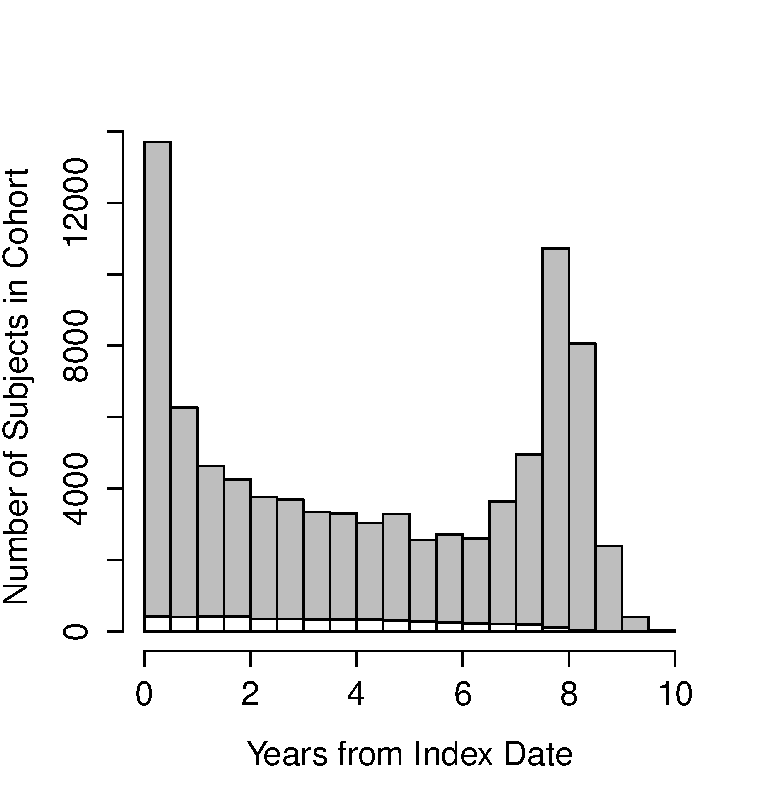
\includegraphics[width=0.50\textwidth]{followup.pdf}
\caption{Distribution of follow-up times, i.e., time from the end of the baseline period until the patient experiences a CV event, the patient disenrolls from the insurance for more than 90 days, or the study ends, in our entire cohort after applying inclusion/ exclusion criteria detailed in Section \ref{sect:studypop}. The number of subjects whose follow-up ends in a CV event are shown in white bars while the number whose follow-up is censored is given by the gray bars.}
\label{figure:followDist}
\end{figure}

\begin{figure}[h]
\centering
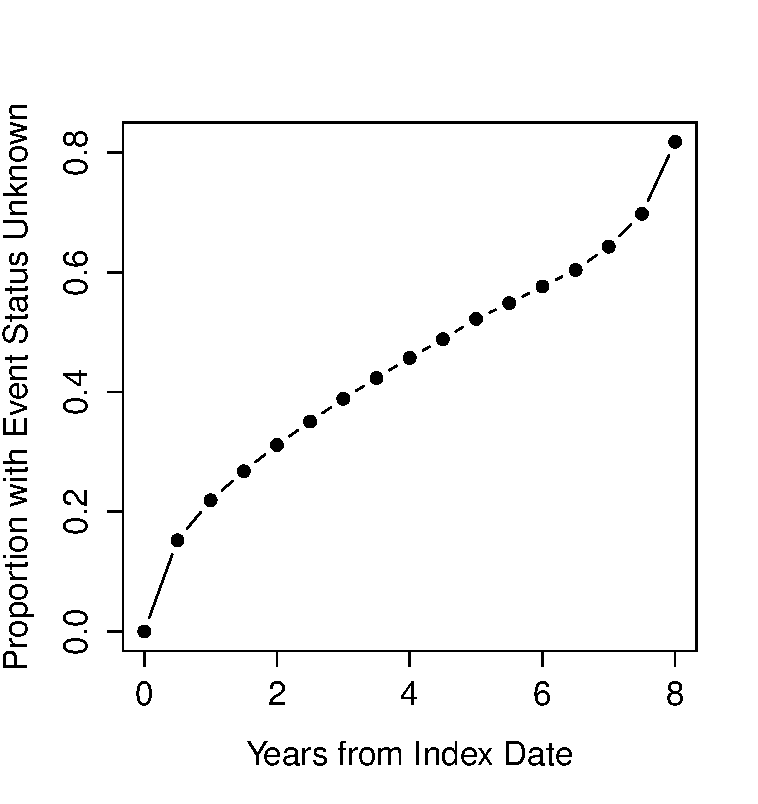
\includegraphics[width=0.50\textwidth]{prop_unknown.pdf}
\caption{Proportion of subjects with unknown $\tau$-year event status as a function of $\tau$, the time from index date in years.}
\label{figure:UnknownEvents}
\end{figure}

%%%
\subsection{Risk factor ascertainment}
\label{sect:riskfactors}

Risk factors used as features in the machine learning models included age, gender, systolic blood pressure (SBP), use of blood pressure medications, cholesterol markers (HDL and total cholesterol), body mass index (BMI), smoking status, and presence/absence of diabetes.  Summary statistics and brief descriptions for the risk factors are given in Table \ref{table:cohortProps}. Missing risk factor values were filled in prior to model fitting using multiple imputation by chained equations \citep{vanBuuren2011} to create a dataset with no mising values; Table \ref{table:cohortProps} displays the percentage of missing values for each risk factor in the original (pre-imputation) data set.

\begin{center}
\begin{table}
\tbl{Distribution of risk factors in the analysis dataset.\label{table:cohortProps}}{%
\begin{tabular}{l|ccl}\hline \noalign{\smallskip}
                          & {\bf{Median (IQR)}}       &   {\bf{\% missing}}                &                                                                          \\
{\bf{Feature Name}}       &      or                   & {\bf{(in}} &  {\bf{Description}}                                                      \\
                          & {\bf{N (\%)}}             &     {\bf{original data)}}              &                                                                          \\ \noalign{\smallskip}\hline\noalign{\smallskip} \hline
{\bf{Gender}}             &                           &                   &                                                                          \\
\ \ \ Female              & 51,530 (59.0)            &  0                &                                                                          \\
\ \ \ Male                &  35,833 (41.0)            &  0                &                                                                          \\
{\bf{Age }}(Years)        & 52      (46  -  60)       &  0                &  Age  at the end of the baseline period                                  \\
{\bf{SBP }}(mm Hg)        & 123     (115 - 133)       &  0                &  Average systolic blood pressure  during baseline period                    \\
{\bf{BMI }}(kg/m$^2$)     & 28.0    (24.7  -  32.3)   &  8               & Body mass index                                                          \\
{\bf{HDL }}(mg/dL)        & 48      (40  -  59)       &  41               &  Final high density lipoprotein during baseline period                  \\
{\bf{Total cholesterol }}(mg/dL)        & 196      (172  -  222)       &  41             &  Final total cholesterol during baseline period                  \\
{\bf{Smoking}}            &                           &                   & Smoking status in EMR                                                    \\
\ \ \ Never or Passive    & 64,335 (73.6)            &   0               &                                                                          \\
\ \ \ Quit                & 9,829  (11.3)             &   0               &                                                                          \\
\ \ \ Current             & 13,199  (15.1)            &   0               &                                                                          \\
{\bf{SBP Meds}}           &                           &                   &  Subject is currently taking SBP medication during baseline period          \\
\ \ \ No                   & 49,165 (56.3)            &   0               &                                                                          \\
\ \ \ Yes                & 38,198 (43.7)             &   0               &                                                                          \\
{\bf{Diabetes}}            &                           &                   & Subject has a current diagnosis of diabetes                                                    \\
\ \ \ No               & 80,921  (92.6)             &   0               &                                                                          \\
\ \ \ Yes    & 6,442 (7.4)            &   0               &                                                                          \\
\noalign{\smallskip}
\hline
\end{tabular}}
\end{table}
\end{center}

\subsection{Events and censoring}

Cardiovascular events were defined as the first recorded stroke, myocardial infarction (MI), or procedure proximal to stroke or MI (e.g., coronary artery bypass surgery, stent for either the coronary arteries or carotid artery) after the baseline period, prior to 5 years of follow-up. This information was obtained from diagnosis codes recorded by physicians or inferred from procedures (such as bypass surgery or stent placement) performed on an individual. In addition to using procedure and diagnosis codes to infer if a CV event occurred, we considered a patient to have experienced a CV event if the cause of death listed on the death certificate included MI or stroke. The total number of first CV events recorded within 5 years of the baseline period was 3,653; the 5-year event rate for the entire analysis cohort calculated via Kaplan-Meier was 6.4\%.

%%%
\section{Models and results} \label{sect:data-analysis}

Subjects who experienced an event within five years were recorded as $E=1$, and those with at least 5 years of event-free follow-up were recorded as $E=0$.  Subjects who were event-free but censored before accruing 5 years of follow-up have $E$ unknown. We applied and evaluated four variants of each of the machine learning techniques described in Section \ref{sect:examples} to our data. The variants differ in their handling of subjects with $E$ unknown:
\begin{enumerate}
\item \textbf{Set $E=0$ if $E$ is unknown}. Techniques using this strategy are denoted with the suffix \emph{-Zero}.
\item \textbf{Discard observations with $E$ unknown}. Techniques using this strategy are given the suffix \emph{-Discard}.
\item \textbf{Use IPCW on observations with $E$ known}. The resulting techniques, as described in Section \ref{sect:examples}, have the suffix \emph{-IPCW}.
\item \textbf{``Split'' observations with $E$ unknown into two observations with $E=1$ and $E=0$ with weights based on marginal survival probability}. The resulting techniques, as described previously, have the suffix \emph{-Split}. \JWcomment{Need to add section describing this}
\end{enumerate}

Results from the Cox proportional hazards model \citep{Cox_1972} are included for comparison. The Cox model is a well-established technique for estimating survival probabilities which has been used as the basis for many CV risk prediction models, including the popular Framingham risk score \citep{DAgostino_2008}. If the Cox regression model is correctly specified, the estimated survival probabilities converge to the true probabilities as the sample size increases.

Model performance was assessed based on the calibration and discrimination metrics described in Section \ref{sec:performanceMetrics}. To calculate the calibration statistic and cNRI, we defined five risk strata based on clinically relevant cutoffs for the risk of experiencing a cardiovascular event within 5 years: 0-5\%, 5-10\%, 10-15\%, 15-20\% and $>$ 20\% \citep{Ridker_2007}. For the cNRI, risk predictions for an individual were considered discordant between two models if the predictions fell in different ranges. Asymptotically, the calibration statistic has a $\chi^2$ distribution with 3 degrees of freedom, so a statistical test for the null hypothesis that a model is well-calibrated would fail to reject at a 5\% significance level if the statistic exceeds 7.81.  All models were fitted using the open-source statistical software program R \citep{RProject}. Code is available from the first author's website, \url{https://sites.google.com/site/dmvock/}.

We now provide some implementation details for the various machine learning techniques.

\subsection{Logistic and Cox regression}

Logistic regression models were defined as
\[
\log \left( \frac{\pi(\mbf{X})}{1 - \pi(\mbf{X})} \right) = \beta_0 + \beta_1 X_1 + \beta_2 X_2 + \dots
\]
where $X_1, X_2, \dots$ are variables representing the (unscaled) risk factors described in Section \ref{sect:riskfactors}. The reported results are for models with a single ``main effect'' term for each predictor (i.e., no interactions or transformations); predictive performance did not markedly improve when second-order interaction terms were included (data not shown). Models were fitted using the \texttt{glm} function in R; IPC weights were incorporated using the \texttt{weights} argument.

The Cox model specifies the relationship between the risk factors and the hazard function $\lambda(t;\mathbf{X}) = f_T(t) / S(t)$, where $f_T$ is the density function and $S$ the survivor function of $T$. Here, we take 
\[
\lambda(t;\mathbf{X}) = \lambda_0(t) \exp(\beta_1 X_1 + \beta_2 X_2 + \dots)
\]
where the risk factors $X_1, X_2, \dots$ are the same as for the logistic regression model. The resulting model is fairly similar to the one used to compute the Framingham risk score, providing an established standard against which to compare our models' calibration and reclassification performance. 

\subsection{Bayesian networks}

Figure \ref{figure:BayesNet} displays the structure of the Bayesian network that we used to construct our prediction models. The structure was determined by combining known relationships from the medical literature with input from our clinical colleagues. As noted in Section \ref{sect:BN}, it is possible to use IPCW to account for censoring when building and comparing different graph structures.

\begin{figure*}[h]
\centering
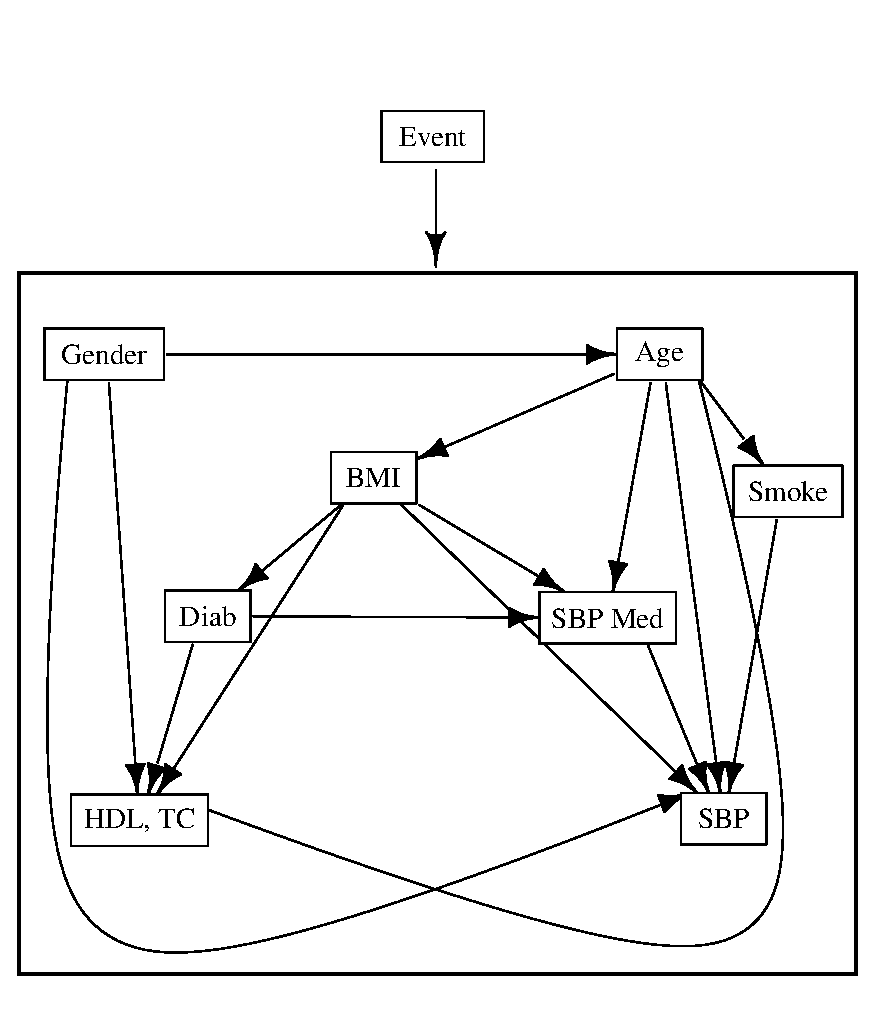
\includegraphics[width=0.75\textwidth]{bayesian_network_joint.pdf}
\caption{The graphical model for our Bayesian network for CV risk prediction.  The figure includes the structure of risk factors, conditioned on the CV event status.  In particular, nodes represent input variables and edges represent conditional dependencies between the variables. The grey edge between subgraphs indicates an edge from every node in the source subgraph to every node in the destination subgraph or node.  That is, the reader should assume that our outcome variable (CV Event) is connected to every node in the graph.  Features in the same Nodes indicate those features are modeled jointly. The full description of each of the features appears in Section~\ref{sec:data}. {\em Smoke}: current smoking status of patient; {\em BMI}: body mass index of patient; {\em Diab}: indicator for whether or not patient is diabetic {\em SBP}: systolic blood pressure; {\em SBP Med}: indicator for whether or not patient is prescribed blood pressure medication; {\em HDL}: high density lipoprotein; {\em TC}: total cholesterol (note that HDL and TC are modelled jointly).}
\label{figure:BayesNet}
\end{figure*}

Nodes were jointly modeled as described in Section \ref{sect:BN}, assuming a single multivariate Normal distribution for each jointly modeled set of continuous codes ($M=1$ in Equation \eqref{eq:JoinDistComps2}). Risk factors were scaled to zero mean and unit variance prior to fitting the model, which was custom-coded in Matlab. Code is available upon request.

\subsection{Classification trees}

Classification trees were built using the \texttt{rpart} package in \texttt{R}, which implements the classification and regression trees described in \citet{Breiman1984classification}. Nodes are split based on the Gini loss criterion; the loss matrix was modified to give 10 times as much weight to incorrect non-event predictions among those experiencing events than the reverse, to induce additional splits and improve discrimination among the large fraction of the population with a relatively low (e.g., $< 5\%$) 5-year CV event risk. The minimum number of subjects in each terminal node was fixed at 200. Risk factors were not scaled prior to fitting the tree. In this illustrative example, no explicit pruning was performed, though this would be advisable to optimize performance in practice. IPC weights were incorporated via the \texttt{weights} argument in \texttt{rpart}, which treats them as case weights.

%%%%
\section{Results} \label{sect:data-analysis2}

The full training dataset consists of 65,522 patients (75\%) drawn at random from the analysis cohort. 52\% were censored prior to five years, so that \emph{-Discard} models were trained on 31,345 subjects. The performance of all models is evaluated based on the risk predictions of the remaining 21,841 patients not included in any training set. 

\begin{table}[h]
\centering
\tbl{Calibration statistic and C-index of versions of classification trees ({\em{Tree}}), k-nearest neighbors ({\em{k-NN}}), Bayesian network models ({\em{Bayes}}), logistic regression ({\em{Logistic}}), generalized additive models ({\em{GAM}}), and Cox proportional hazards model ({\em{Cox}}) evaluated on the hold-out test set. {\em{Predicted event rate}}: Average predicted probability of experiencing a CV event within 5 years;  {\em{Calibration}}: calibration test statistic $K$; {\em{C-index}}: Concordance index adapted for censoring;  \label{table:calib-cindex} }{%
\begin{tabular}{lccc}
& \bf{Predicted} & & \\
\bf{Method} & \bf{event rate (\%)} & \bf{Calibration} & \bf{C-Index} \\
  \hline
\bf{Tree} &  &  &  \\
  \hspace{0.20in} -IPCW & 5.41 & 12.74 & 0.788 \\
  \hspace{0.20in} -Discard & 7.13 & 76.92 & 0.784 \\
  \hspace{0.20in} -Zero & 4.19 & 125.76 & 0.784 \\
  \hspace{0.20in} -Split & 6.42 & 289.54 & 0.782 \\
   \hline
\bf{k-NN} &  &  &  \\
  \hspace{0.20in} -IPCW & 5.27 & 10.24 & 0.787 \\
  \hspace{0.20in} -Discard & 7.07 & 49.11 & 0.793 \\
  \hspace{0.20in} -Zero & 4.11 & 85.64 & 0.788 \\
  \hspace{0.20in} -Split & 6.37 & 106.60 & 0.787 \\
   \hline
\bf{Bayes} &  &  &  \\
  \hspace{0.20in} -IPCW & 5.62 & 6.18 & 0.802 \\
  \hspace{0.20in} -Discard & 7.40 & 76.82 & 0.802 \\
  \hspace{0.20in} -Zero & 4.26 & 80.16 & 0.800 \\
  \hspace{0.20in} -Split & 6.49 & 194.56 & 0.801 \\
   \hline
\bf{Logistic} &  &  &  \\
  \hspace{0.20in} -IPCW & 5.40 & 4.85 & 0.801 \\
  \hspace{0.20in} -Discard & 7.14 & 63.92 & 0.801 \\
  \hspace{0.20in} -Zero & 4.18 & 83.78 & 0.799 \\
  \hspace{0.20in} -Split & 6.42 & 150.46 & 0.797 \\
   \hline
\bf{GAM} &  &  &  \\
  \hspace{0.20in} -IPCW & 5.47 & 6.96 & 0.805 \\
  \hspace{0.20in} -Discard & 7.22 & 67.57 & 0.804 \\
  \hspace{0.20in} -Zero & 4.17 & 83.04 & 0.801 \\
  \hspace{0.20in} -Split & 6.42 & 233.07 & 0.802 \\
   \hline
\bf{Cox} &  &  &  \\
   & 5.69 & 8.80 & 0.801 \\
   \hline
  \end{tabular}
  }
\end{table}

\begin{figure*}[h]
	\centering
	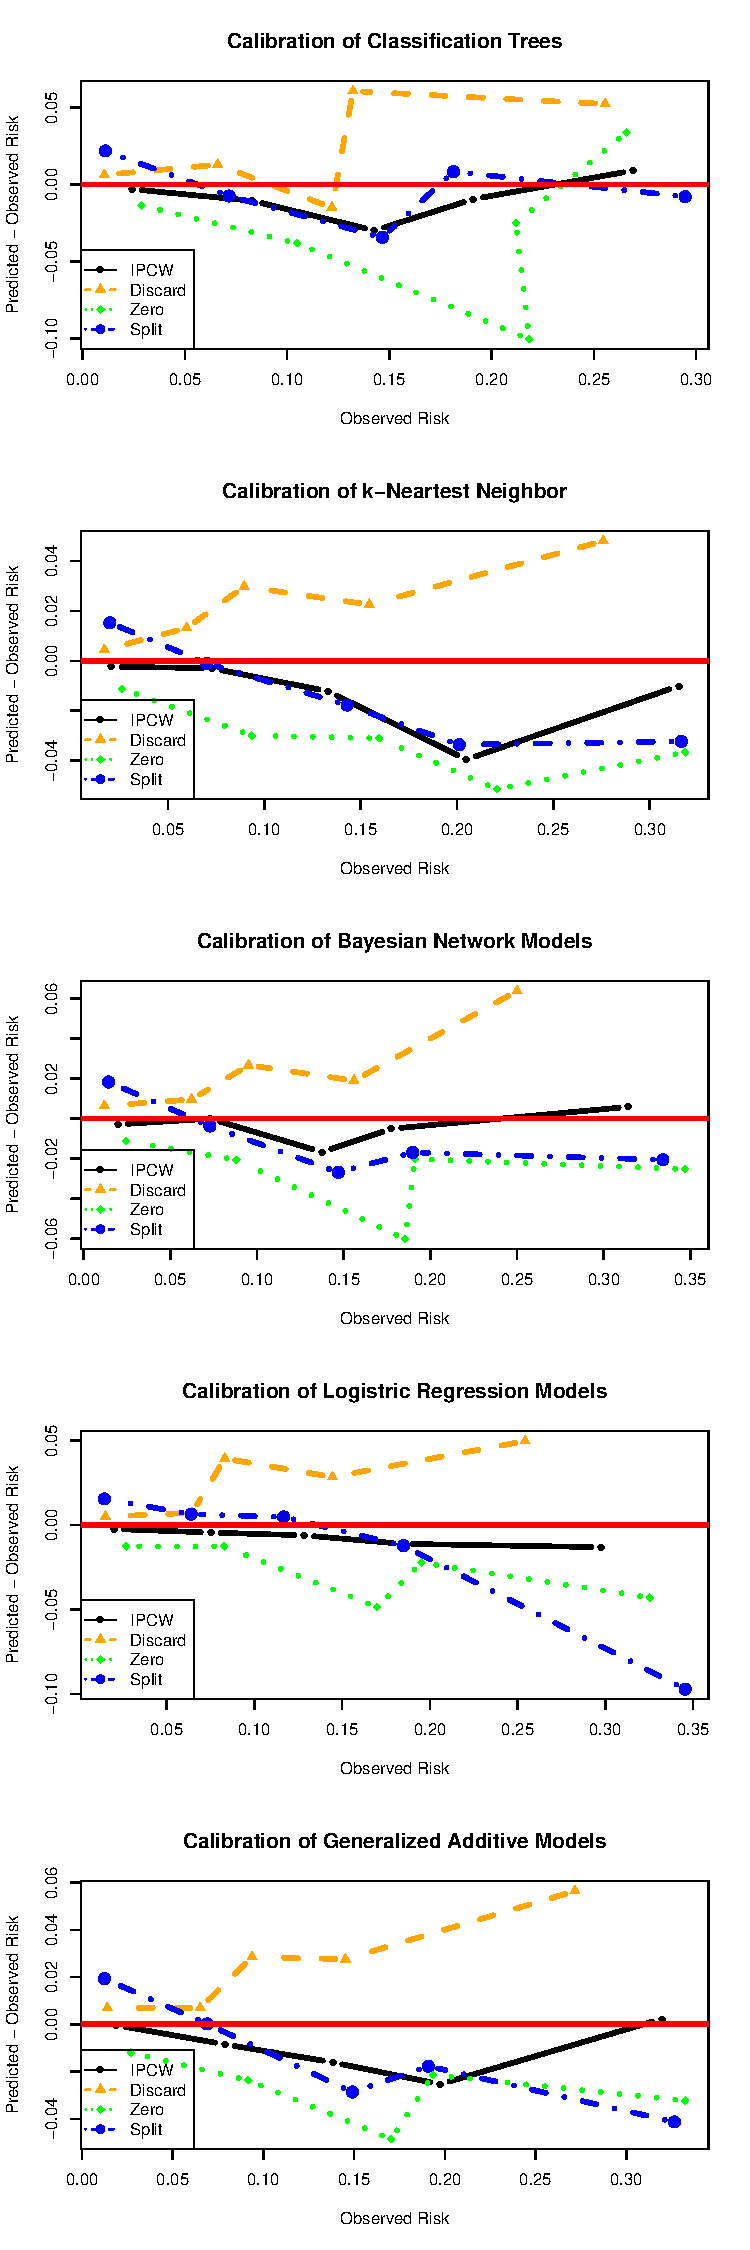
\includegraphics[width=0.45\textwidth]{calibration_plots.pdf}
	\caption{Test.}
	\label{figure:calib}
\end{figure*}

Table \ref{table:calib-cindex} shows how different approaches to handling censored observations affect the predicted event rate, calibration statistic, and C-index of the techniques described in Section \ref{sect:examples}. Figure \ref{figure:calib} displays calibration plots which compare predicted to empirical (computed from Kaplan-Meier) risks across bins defined by the predicted risk. From Table~\ref{table:calib-cindex} and Figure \ref{figure:calib}, it is clear that the \emph{-Discard}, \emph{-Zero}, and \emph{-Split} variants of each technique are poorly calibrated. As expected, the \emph{-Discard} and \emph{-Split} approaches over-estimate risk and the \emph{-Zero} approaches underestimate it, both overall and within subgroups. The \emph{-IPCW} versions are generally well-calibrated, with predicted event rate and calibration similar to the Cox model. Reclassification performance is not dramatically affected by the way in which censoring is handled, with small gains (change in C-index of $< 0.005$) in most techniques due to IPCW. 

Table \ref{table:cNRI} compares the net reclassification improvement for the IPCW versions of various techniques, along with the Cox model. We do not consider cNRIs for the \emph{-Discard}, \emph{-Zero} and \emph{-Discard} variants as recent papers \citep{Pepe_2011} have shown that the NRI can be a very misleading statistic when comparing poorly calibrated models. In almost all cases, reclassification performance as measured by cNRI is similar across the techniques, which is consistent with the C-index results in Table \ref{table:calib-cindex}.

\begin{table}[h]
	\centering
	\tbl{Net reclassification (cNRI) comparisons for IPC weighted versions of classification tree, k-nearest neighbors, Bayesian network, logistic regression, generalized additive model and Cox proportional hazards model, evaluated on the hold-out test set. Positive numbers indicate that the bolded technqiue correctly reclassifies subjects more frequently than the technique preceded by ``vs.''.  \emph{cNRI (Events)} and \emph{cNRI (Non-Events)} give the reclassification improvement among those who did and did not experience events, and \emph{cNRI (Overall)} is their sum. \emph{cNRI (Overall Weighted)} is a weighted sum where the reclassification performance among Events and Non-Events is weighted according to the event and non-event probabilities, respectively. \label{table:cNRI} }{
\begin{tabular}{lcccc}
	\hline
	& cNRI (Events) & cNRI (Non-Events) & cNRI (Overall) & cNRI (Overall Weighted) \\
	\hline
			\bf{Tree} &  &  & & \\
			\hspace{0.20in} vs. kNN & -0.003 & 0.048 & 0.045 & 0.045 \\
			\hspace{0.20in} vs. Bayes & -0.064 & 0.058 & -0.006 & 0.050 \\
			\hspace{0.20in} vs. Logistic & -0.065 & 0.045 & -0.020 & 0.038 \\
			\hspace{0.20in} vs. GAM & -0.056 & 0.030 & -0.026 & 0.024 \\
			\hspace{0.20in} vs. Cox & -0.102 & 0.061 & -0.041 & 0.051 \\
			\hline
			\bf{k-NN} &  &  &  & \\
			\hspace{0.20in} vs. Bayes & -0.065 & 0.015 & -0.050 & 0.009 \\
			\hspace{0.20in} vs. Logistic & -0.108 & 0.009 & -0.099 & 0.001 \\
			\hspace{0.20in} vs. GAM & -0.069 & -0.013 & -0.082 & -0.016 \\
			\hspace{0.20in} vs. Cox & -0.159 & 0.031 & -0.128 & 0.018 \\
			\hline
			\bf{Bayes} &  &  &  & \\
			\hspace{0.20in} vs. Logistic & -0.013 & -0.017 & -0.030 & -0.017 \\
			\hspace{0.20in} vs. GAM & 0.028 & -0.040 & -0.012 & -0.035 \\
			\hspace{0.20in} vs. Cox & -0.060 & 0.002 & -0.058 & -0.002 \\
			\hline
			\bf{Logistic} &  &  &  & \\			
			\hspace{0.20in} vs. GAM & 0.037 & -0.022 & 0.015 & -0.018 \\
			\hspace{0.20in} vs. Cox & -0.053 & 0.021 & -0.031 & 0.017\\
			\hline
			\bf{GAM} &  &  &  & \\			
			\hspace{0.20in} vs. Cox & -0.085 & 0.043 & -0.043 & 0.035 \\
			\hline
		\end{tabular}
	}
\end{table}

While the machine learning techniques we illustrated did not substantially outperform the Cox model, we note that in the context of CV risk prediction the Cox model sets a high standard as with the given risk factors it has been shown repeatedly to have excellent calibration and reclassification performance \citep{DAgostino_2001,Eichler_2007}.  However, the IPCW technique is applicable to a wide range of situations where follow-up data are censored and the Cox model may not perform as well as more flexible machine learning techniques.

\section{Discussion}

We have proposed a general-purpose technique for improving the performance of machine learning methods when the binary class indicator is unknown for a subset of individuals due to censoring. Though motivated by an example in electronic health data, our technique is generally applicable to any situation where event outcomes are subject to censoring. For example, in economics, one might wish to predict whether recently-unemployed individuals will be re-hired within a fixed time period, an outcome which is likely to be censored in most feasible study designs. In our context, we plan to incorporate this technique into a point-of-care clinical decision support system, which will provide more accurate cardiovascular risk predictions for patients based on their individual health history.

\subsection{Limitations}

The statistical validity of IPCW rests on several assumptions, in particular that the censoring time is independent of both the event time and patient features. This is a plausible assumption for EHD, where censoring typically occurs for reasons unrelated to a person's health status, but the assumption is much less plausible in other contexts. For example, if data were collected from a small regional hospital, patients with severe health problems might be censored because they went to a larger facility to seek care. In practice, it is unlikely that the independence assumption is satisfied exactly, and it is an open question how the degree to and manner in which the assumption is violated affects the performance of IPCW techniques.

The benefits of IPCW also depend on the proportion of subjects who are censored and hence have an undetermined event indicator. In our data, approximately half of subjects were censored before 5 years, a level of censoring which is amenable to IPCW. When few subjects (e.g., $< 10\%$) are censored, the gains of IPCW over ``naive'' techniques will be modest. When the vast majority (e.g., $> 90\%$) are censored, only a small fraction of subjects will be used in the analysis, with many having large and highly variable weights.

\subsection{Extensions and Future Work}

We have provided several examples of how to incorporate IPCW into established machine learning techniques. There are, of course, a wide variety of ML algorithms which we did not implement, but the simplicity of the IPCW approach means that it can be adapted to a wide range of existing tools. Indeed, due to IPCW's generality of ease and implementation, it would be relatively straightforward to develop ensemble-based risk prediction tools to apply to censored data. For instance, given an implementation of IPCW decision trees, constructing an IPCW random forest is quite simple.

Most of the analyses reported in this paper were performed using implementations of these techniques in standard statistical software, but support for a ``weights'' argument is not universal across popular ML packages. Even implementations which do allow for weights to be specified may not use them consistently, e.g., they will be used for training the model but not for tuning parameter selection. In ongoing work, we are developing more general resampling-based approaches which will allow IPCW analyses to be performed using ML software which lacks the capacity to handle user-specified weights.

% Acknowledgments
%\begin{acks}
%The authors would like to thank Dr. Maura Turolla of Telecom
%Italia for providing specifications about the application scenario.
%\end{acks}

% Bibliography
\bibliographystyle{ACM-Reference-Format-Journals}
\bibliography{ML_for_censored_refs}

% History dates
%\received{February 2007}{March 2009}{June 2009}

% Electronic Appendix
%\elecappendix

%\medskip
%
%\section{This is an example of Appendix section head}
%
%Channel-switching time is measured as the time length it takes for
%motes to successfully switch from one channel to another. This
%parameter impacts the maximum network throughput, because motes
%cannot receive or send any packet during this period of time, and it
%also affects the efficiency of toggle snooping in MMSN, where motes
%need to sense through channels rapidly.
%
%By repeating experiments 100 times, we get the average
%channel-switching time of Micaz motes: 24.3 $\mu$s. We then conduct
%the same experiments with different Micaz motes, as well as
%experiments with the transmitter switching from Channel 11 to other
%channels. In both scenarios, the channel-switching time does not have
%obvious changes. (In our experiments, all values are in the range of
%23.6 $\mu$s to 24.9 $\mu$s.)
%
%\section{Appendix section head}
%
%The primary consumer of energy in WSNs is idle listening. The key to
%reduce idle listening is executing low duty-cycle on nodes. Two
%primary approaches are considered in controlling duty-cycles in the
%MAC layer.

\end{document}
